\documentclass[11pt]{article}
% arXiv categories: quant-ph (primary), cs.DC, physics.comp-ph
\usepackage[margin=1in]{geometry}
\usepackage{amsmath}
\usepackage{amssymb}
\usepackage{algorithm}
\usepackage{algpseudocode}
\usepackage{graphicx}
\usepackage{booktabs}
\usepackage{hyperref}
\usepackage{xcolor}
\usepackage{listings}

% Code listing style
\lstset{
    language=Python,
    basicstyle=\ttfamily\small,
    keywordstyle=\color{blue},
    commentstyle=\color{gray},
    stringstyle=\color{red},
    numbers=left,
    numberstyle=\tiny\color{gray},
    frame=single,
    breaklines=true,
    captionpos=b
}

\title{Parallelizing the Variational Quantum Eigensolver: \\
From JIT Compilation to Multi-GPU Scaling}

\author{
R. Malarchick\textsuperscript{1} and A. Steed\textsuperscript{1} \\[0.5em]
\textsuperscript{1}Department of Physical Sciences, Embry-Riddle Aeronautical University, \\
Daytona Beach, FL 32114, USA \\[0.5em]
\texttt{rylan1012@gmail.com, steeda1@my.erau.edu}
}

\date{January 2026; revised October 2026}

\begin{document}

\maketitle

\begin{abstract}
    The Variational Quantum Eigensolver (VQE) is a hybrid quantum-classical algorithm for ground-state energies of molecular systems. We compute the potential energy surface of the hydrogen molecule (H$_2$) at 100 bond lengths with PennyLane on the ERAU Vega cluster (AMD EPYC 9654 CPUs, 4 NVIDIA H100 GPUs) and compare a serial baseline, an Optax and Catalyst JIT version, a \texttt{lightning.gpu} version, and an MPI version. Early stopping, a larger learning rate, and warm starts reduce the iteration count from 30,000 to 7,033 and the runtime from 593.95~s to 143.80~s, while the time per iteration stays between 0.0198~s and 0.0204~s. At 4 qubits, \texttt{lightning.gpu} lowers the time per iteration to 0.0145~s. MPI runs with 2 to 32 ranks finish in 8.45~s to 5.04~s; the serial and MPI jobs ran under different core allocations, so we do not report their ratio as a parallel speedup. In a 4 to 26 qubit study with different CPU and GPU software stacks, the CPU/GPU time ratio ranges from 3.5 to 81.5. One H100 runs up to 29 qubits.
\end{abstract}

\section{Introduction}

\subsection{Background}

Quantum chemistry computes molecular structure, reaction pathways, and material properties from first principles. A central problem is the ground-state energy and wavefunction of a molecule. The cost of an exact calculation grows exponentially with the number of orbitals, which limits exact classical methods to small molecules.

The Variational Quantum Eigensolver (VQE) is a hybrid quantum-classical algorithm \cite{peruzzo2014} designed for noisy near-term devices. A parameterized quantum circuit (the ansatz) prepares trial wavefunctions, and a classical optimizer adjusts the parameters to minimize the energy.

We study the hydrogen molecule (H$_2$), the simplest neutral molecule and a standard benchmark for quantum chemistry methods. Its potential energy surface has an equilibrium bond length and a dissociation limit.

\subsection{Issues and Questions to be Addressed}

This work addresses two questions:

\begin{enumerate}
    \item \textbf{Quantum Chemistry}: Can VQE accurately compute the H$_2$ potential energy surface using a minimal ansatz with a single variational parameter?

    \item \textbf{High Performance Computing}: How do JIT compilation, GPU simulation, and MPI distribution change the runtime of the H$_2$ scan on an HPC node?
\end{enumerate}

The serial implementation provides the baseline for the other implementations.

\subsection{Related Work}

Peruzzo et al.~\cite{peruzzo2014} first demonstrated VQE experimentally on a photonic quantum processor. Since then, ansatz design has been a major focus: the Unitary Coupled Cluster (UCC) ansatz~\cite{romero2018} is now standard for molecular simulations, while hardware-efficient ansatzes~\cite{kandala2017} reduce circuit depth on noisy devices.

Several software tools speed up the classical simulation of variational algorithms. PennyLane~\cite{bergholm2018} provides automatic differentiation for quantum circuits, and its Lightning backend~\cite{pennylane_lightning} provides compiled state-vector simulation. NVIDIA's cuQuantum~\cite{cuquantum2023} targets multi-GPU simulation, and JAX~\cite{jax2018} enables JIT compilation for numerical code.

MPI parallelization of quantum chemistry is well-established~\cite{valiev2010}. We apply the same distribution of independent work to VQE and measure JIT compilation, GPU simulation, and MPI distribution on one HPC node with four H100 GPUs. We report each runtime together with its optimizer and stopping settings.

\section{Problem Description}

\subsection{The Molecular Hamiltonian Problem}

The goal is to compute the ground state energy $E_0$ of the H$_2$ molecule as a function of internuclear distance $d$. The electronic Hamiltonian in the Born-Oppenheimer approximation is:

\begin{equation}
    H = -\frac{1}{2}\sum_{i=1}^{2}\nabla_i^2 - \sum_{i=1}^{2}\left(\frac{1}{|\mathbf{r}_i - \mathbf{R}_A|} + \frac{1}{|\mathbf{r}_i - \mathbf{R}_B|}\right) + \frac{1}{|\mathbf{r}_1 - \mathbf{r}_2|} + \frac{1}{d}
\end{equation}

where $\mathbf{r}_i$ are electron positions, $\mathbf{R}_A$ and $\mathbf{R}_B$ are nuclear positions separated by distance $d$, and atomic units are used.

We project this Hamiltonian onto the minimal STO-3G basis and map it to qubit operators with the Jordan-Wigner transformation.

\subsection{Computational Task}

The specific computational problem is:

\begin{itemize}
    \item \textbf{Input}: Set of bond lengths $\{d_1, \ldots, d_{100}\}$ uniformly spaced from 0.35 to 3.0 \AA
    \item \textbf{Output}: Ground state energies $\{E_1, \ldots, E_{100}\}$ at each bond length
    \item \textbf{Constraint}: Each energy must converge (the baseline runs 300 VQE iterations per bond length)
    \item \textbf{Objective}: Minimize total wall-clock time while maintaining accuracy
\end{itemize}

Each bond length requires:
\begin{itemize}
    \item Hartree-Fock calculation to generate molecular Hamiltonian
    \item Up to 300 optimization steps, each with a cost and a gradient evaluation
    \item Parameter updates via Adam optimizer
\end{itemize}

On the cluster, the baseline runs 30,000 optimization steps in total (Section~\ref{sec:parallel_results}).

\section{Model Formulation}

\subsection{The Variational Principle}

VQE relies on the variational principle: for any normalized trial wavefunction $|\psi(\theta)\rangle$ with parameters $\theta$, the energy expectation value is bounded below by the ground-state energy,

\begin{equation}
    E(\theta) = \langle \psi(\theta) | H | \psi(\theta) \rangle \geq E_0
\end{equation}

where $E_0$ is the ground-state energy and $H$ is the molecular Hamiltonian. The minimum of $E(\theta)$ is an upper bound on $E_0$, and it is close to $E_0$ when the ansatz can represent a state close to the ground state.

\subsection{Molecular Hamiltonian in Second Quantization}

For the H$_2$ molecule, the electronic Hamiltonian in second quantization is:

\begin{equation}
    H = \sum_{i,j} h_{ij} a_i^\dagger a_j + \frac{1}{2}\sum_{i,j,k,\ell} h_{ij k\ell} a_i^\dagger a_j^\dagger a_k a_\ell
\end{equation}

where:
\begin{itemize}
    \item $h_{ij}$ are one-electron integrals (kinetic energy and nuclear attraction)
    \item $h_{ij k\ell}$ are two-electron integrals (electron-electron repulsion)
    \item $a_i^\dagger, a_i$ are fermionic creation and annihilation operators
\end{itemize}

PennyLane computes these integrals over the Hartree-Fock molecular orbitals of the STO-3G basis and maps the Hamiltonian to Pauli operators on 4 qubits with the Jordan-Wigner transformation.

\subsection{Quantum Circuit Ansatz}

The trial wavefunction is prepared using a parameterized quantum circuit:

\begin{equation}
    |\psi(\theta)\rangle = U(\theta) |\text{HF}\rangle
\end{equation}

where:
\begin{itemize}
    \item $|\text{HF}\rangle = |1100\rangle$ is the Hartree-Fock reference state (both electrons in lowest spatial orbital with opposite spins)
    \item $U(\theta)$ is a unitary operator implemented as a double excitation gate
\end{itemize}

The double excitation gate is:

\begin{equation}
    U(\theta) = \exp\left(-i\frac{\theta}{2}(a_0^\dagger a_1^\dagger a_2 a_3 - a_3^\dagger a_2^\dagger a_1 a_0)\right)
\end{equation}

This ansatz describes the dominant correlation in H$_2$, the double excitation of both electrons from the bonding to the antibonding orbital, with a single parameter $\theta$. In simulation, the gate is a parameterized unitary applied to the $2^N$-dimensional state vector, and the optimization is a one-parameter minimization of an expectation value.

\subsection{Optimization Problem}

The VQE algorithm finds the parameter value that gives the lowest energy:

\begin{equation}
    \theta^* = \arg\min_\theta E(\theta) = \arg\min_\theta \langle \psi(\theta) | H | \psi(\theta) \rangle
\end{equation}

The baseline uses the Adam optimizer with:
\begin{itemize}
    \item Learning rate: $\alpha = 0.01$
    \item Iterations per bond configuration: $N_{\text{iter}} = 300$ (baseline; Section~\ref{sec:parallel_results} lists the settings of the other implementations)
    \item Initial parameter: $\theta_0 = 0$ (starts at Hartree-Fock state)
\end{itemize}

\section{Methods}

\subsection{Problem Structure and Parallelization Opportunities}

The potential energy surface requires $E(\theta^*)$ at $N_b = 100$ bond lengths in the range $[0.35, 3.0]$~\AA. For each bond length $d_i$, the baseline performs four steps:

\begin{enumerate}
    \item Generate molecular Hamiltonian $H(d_i)$ using Hartree-Fock
    \item Initialize variational parameters $\theta_0 = 0$
    \item Optimize: $\theta^*_i = \text{Adam}(E(\theta), \theta_0, N_{\text{iter}} = 300)$
    \item Store ground state energy $E_i = E(\theta^*_i)$
\end{enumerate}

The bond lengths are independent of each other, so the scan is embarrassingly parallel:

\begin{equation}
    E_i = f(d_i) \quad \text{for } i = 1, \ldots, 100
\end{equation}

where $f$ is the VQE optimization procedure.

\subsection{Serial Algorithm Implementation}

The baseline serial implementation follows Algorithm~\ref{alg:serial}.

\begin{algorithm}
    \caption{Serial VQE for H$_2$ Potential Energy Surface}
    \label{alg:serial}
    \begin{algorithmic}[1]
        \State \textbf{Input:} Bond lengths $\{d_1, \ldots, d_{100}\}$
        \State \textbf{Output:} Energies $\{E_1, \ldots, E_{100}\}$
        \State
        \State Initialize quantum device: \texttt{lightning.qubit} with 4 qubits
        \State Define ansatz with Hartree-Fock initialization
        \State
        \For{$i = 1$ to $100$}
        \State Generate $H(d_i)$ using Hartree-Fock (STO-3G basis)
        \State $\theta \gets 0$
        \State Initialize Adam optimizer with $\alpha = 0.01$
        \For{$j = 1$ to $300$}
        \State $E \gets \langle \psi(\theta) | H(d_i) | \psi(\theta) \rangle$ \Comment{Quantum circuit evaluation}
        \State $\nabla_\theta E \gets$ compute gradient (PennyLane default method for \texttt{lightning.qubit})
        \State $\theta \gets \text{Adam\_step}(\theta, \nabla_\theta E)$
        \EndFor
        \State $E_i \gets E(\theta)$ \Comment{Store converged energy}
        \EndFor
        \State \Return $\{E_1, \ldots, E_{100}\}$
    \end{algorithmic}
\end{algorithm}

\textbf{Implementation Details:}
\begin{itemize}
    \item \textbf{Software Versions}: Python 3.12, PennyLane 0.43.1, PennyLane-Catalyst 0.13.0, JAX 0.6.2, Optax 0.2.6, CUDA 11.8, OpenMPI 4.x
    \item \textbf{Basis Set}: STO-3G minimal basis (4 spin-orbitals $\rightarrow$ 4 qubits)
    \item \textbf{Hamiltonian Method}: DHF (built-in Hartree-Fock solver)
    \item \textbf{Device}: PennyLane Lightning simulator (CPU: \texttt{lightning.qubit}, GPU: \texttt{lightning.gpu})
    \item \textbf{Gradient Method}: Automatic differentiation via PennyLane/Catalyst
\end{itemize}

\subsection{Computational Complexity}

A state-vector simulator stores $2^n$ amplitudes for $n$ qubits and applies each gate in $O(2^n)$ operations. For the 4-qubit H$_2$ problem:

\begin{itemize}
    \item State vector dimension: $2^4 = 16$ complex amplitudes
    \item Gradient evaluations: one per optimization step
    \item Optimization steps per bond length: up to 300
    \item Total optimization steps: up to 30,000
\end{itemize}

\subsection{Proposed Parallelization Approaches}

Before the runs, we planned two parallelization approaches and recorded the expected gains.

\subsubsection{Phase 1: JIT Compilation with JAX}

\textbf{Method}: Apply Catalyst just-in-time (JIT) compilation to the cost function using JAX integration in PennyLane.
Optax, a JAX-compatible optimizer library, is used in place of PennyLane's built-in Adam optimizer.

\begin{lstlisting}[caption={Sketch of a JIT-compiled cost function with Optax. The implementation compiles the whole loop with Catalyst \texttt{@qjit}.}]
@jax.jit
@qml.qnode(dev, interface="jax")
def cost_fn(params):
    ansatz(params)
    return qml.expval(H)

# Optimization step
grads = jax.grad(cost_fn)(params)
updates, opt_state = optimizer.update(grads, opt_state)
params = optax.apply_updates(params, updates)
\end{lstlisting}

\textbf{Expected speedup (planned, before the runs)}: 2--5$\times$ from:
\begin{itemize}
    \item Pre-compiling the circuit and optimization for faster execution
    \item Combining operations to reduce memory access time
    \item Computing gradients more efficiently using vector operations
\end{itemize}

\subsubsection{Phase 2: Distributed-Memory Parallelism}

\textbf{Method}: Use OpenMPI with \texttt{mpi4py} to parallelize the outer loop over bond lengths.

\begin{lstlisting}[caption={MPI scatter-gather pattern for embarrassingly parallel VQE.}]
from mpi4py import MPI
comm = MPI.COMM_WORLD
rank, size = comm.Get_rank(), comm.Get_size()

if rank == 0:
    bond_lengths = np.linspace(0.35, 3.0, 100)
    chunks = np.array_split(bond_lengths, size)
else:
    chunks = None

my_chunk = comm.scatter(chunks, root=0)
my_results = [run_vqe(d) for d in my_chunk]
all_results = comm.gather(my_results, root=0)
\end{lstlisting}

Each process runs JIT-compiled VQE independently on its assigned subset of bond lengths, with results gathered to the root process for aggregation.

\textbf{Expected speedup (planned, before the runs)}: $0.8p$ for $p$ cores, below the ideal $p$ because of communication and the JIT compilation on each rank.

\subsubsection{Choice of MPI over Ray}

We first considered the Ray framework for its task-based API. The Ray pip package failed to install alongside PennyLane-Catalyst because of conflicting transitive dependencies, and we did not resolve the version constraints. We therefore used MPI through \texttt{mpi4py}. OpenMPI is installed on the Vega cluster, \texttt{mpi4py} installed without conflicts next to PennyLane, Catalyst, and JAX, and the static split of 100 bond lengths needs no dynamic task scheduling.

\subsection{Performance Prediction Model}
\label{sec:prediction}

Amdahl's law predicts the strong-scaling speedup with $p$ processors:

\begin{equation}
    S_p = \frac{1}{f_s + \frac{f_p}{p}}
\end{equation}

where:
\begin{itemize}
    \item $f_s \approx 0.05$ is the assumed serial fraction (initialization, I/O, plotting)
    \item $f_p \approx 0.95$ is the assumed parallel fraction (VQE optimizations)
\end{itemize}

Table~\ref{tab:predictions} lists the predicted speedups.

\begin{table}[h]
    \centering
    \begin{tabular}{lrr}
        \toprule
        \textbf{Processors} & \textbf{Ideal Speedup} & \textbf{Predicted Speedup} \\
        \midrule
        4                   & 4.0$\times$            & 3.48$\times$               \\
        8                   & 8.0$\times$            & 5.93$\times$               \\
        16                  & 16.0$\times$           & 9.14$\times$               \\
        40                  & 40.0$\times$           & 13.56$\times$              \\
        \bottomrule
    \end{tabular}
    \caption{Predicted parallel speedup using Amdahl's law with $f_s = 0.05$.}
    \label{tab:predictions}
\end{table}

\section{Solution}

\subsection{Serial Implementation Results}

The serial VQE implementation computes the H$_2$ potential energy surface across 100 bond lengths. Table~\ref{tab:serial_performance} lists the metrics of a preliminary run with 8,000 circuit evaluations, a smaller configuration than the 30,000-evaluation cluster runs in Section~\ref{sec:parallel_results}. The two sets of numbers are not comparable.

\begin{table}[h]
    \centering
    \begin{tabular}{lr}
        \toprule
        \textbf{Metric}           & \textbf{Value} \\
        \midrule
        Total Runtime             & 50.64 seconds  \\
        Time per Bond Length      & 1.27 seconds   \\
        Time per VQE Iteration    & 6.3 ms         \\
        Circuit Evaluations/sec   & 157.98         \\
        Total Circuit Evaluations & 8,000          \\
        \bottomrule
    \end{tabular}
    \caption{Preliminary serial run (8,000 circuit evaluations).}
    \label{tab:serial_performance}
\end{table}

The potential energy curve has the expected shape for H$_2$:
\begin{itemize}
    \item Repulsive wall at short bond lengths ($d < 0.74$~\AA)
    \item Equilibrium bond length near $d_{\text{eq}} \approx 0.74$ \AA
    \item Dissociation to separated atoms at large distances ($d > 2.5$ \AA)
\end{itemize}

Figure~\ref{fig:serial_pes} shows the computed potential energy surface.

\begin{figure}[h]
    \centering
    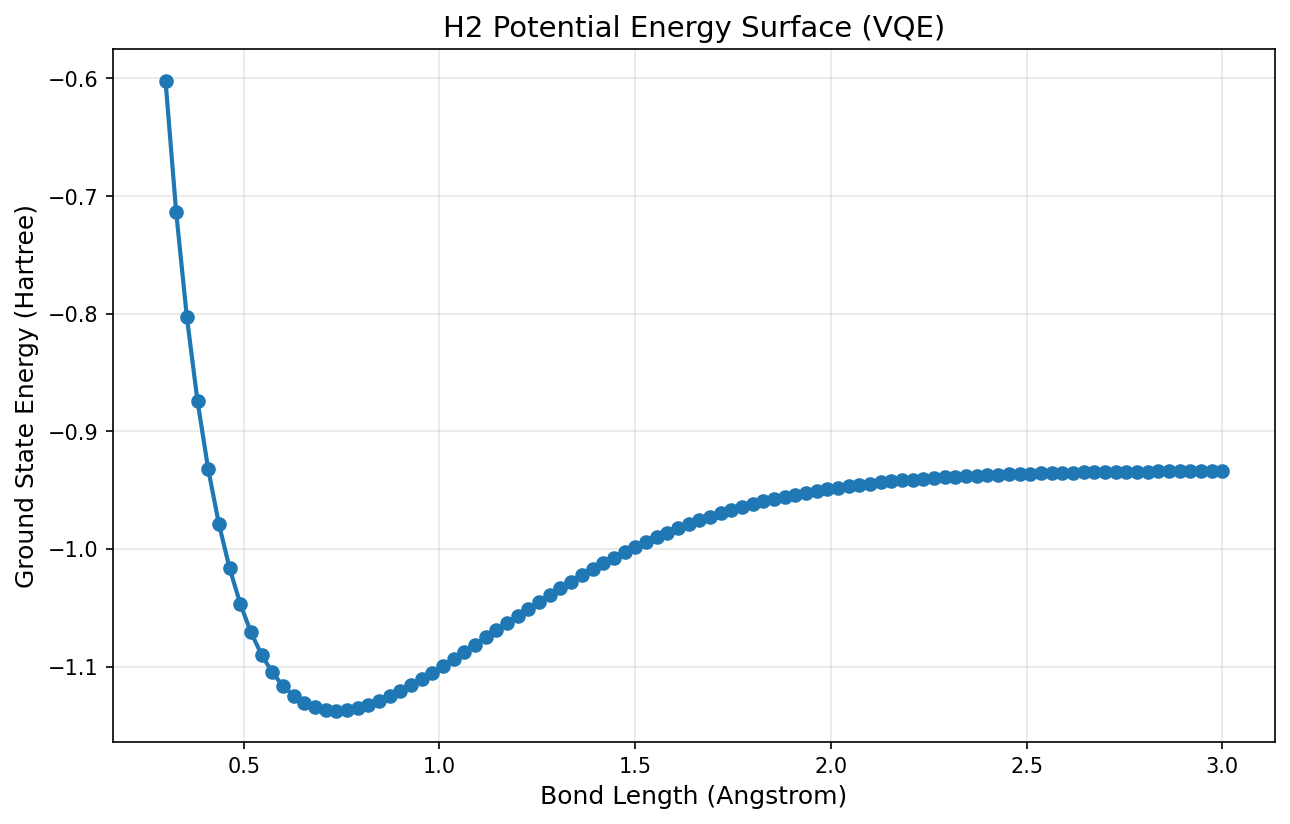
\includegraphics[width=0.8\textwidth]{../results/main_study/vqe_results.png}
    \caption{H$_2$ potential energy surface from the serial VQE implementation, with the minimum near 0.74~\AA\ and the approach to the dissociation limit at large bond lengths.}
    \label{fig:serial_pes}
\end{figure}

\subsection{Parallel Implementation Results}
\label{sec:parallel_results}

We ran all implementations on the ERAU Vega HPC cluster (AMD EPYC 9654 CPUs, 4 NVIDIA H100 GPUs). Every H$_2$ run scans the same 100 bond lengths with at most 300 VQE iterations per bond length. The baseline always runs 300 iterations. The Optax versions stop earlier when the energy converges (Implementation~2).

\subsubsection{Hardware Platform}

\textbf{Compute Node (gpu01):}
\begin{itemize}
    \item CPU: 2$\times$ AMD EPYC 9654 (96 cores each, 192 cores per node)
    \item Memory: 1.5 TB shared memory
    \item GPU: 4$\times$ NVIDIA H100 PCIe (80 GB each)
    \item Interconnect: InfiniBand HDR
\end{itemize}

\subsubsection{Implementation 1: Serial Baseline with PennyLane}

The serial implementation with PennyLane's AdamOptimizer is the baseline:

\begin{itemize}
    \item \textbf{Runtime}: 593.95 seconds (9.90 minutes)
    \item \textbf{Time per bond length}: 5.94 seconds
    \item \textbf{Framework}: PennyLane 0.43.1 with Lightning CPU backend
\end{itemize}

\subsubsection{Implementation 2: Serial Optax and Catalyst JIT (CPU)}

The second implementation (\texttt{vqe\_serial\_optax.py}) compiles the full optimization loop with Catalyst (\texttt{@qjit}, \texttt{catalyst.grad}, \texttt{catalyst.while\_loop}) and uses the Optax Adam optimizer. It also differs from the baseline in three settings. The learning rate is 0.05 instead of 0.01. The loop stops when the energy changes by less than $10^{-8}$~Ha between steps, with at most 300 steps. Each bond length starts from the optimized parameters of the previous bond length instead of from zero.

\begin{itemize}
    \item \textbf{Runtime}: 143.80 seconds (baseline: 593.95 seconds)
    \item \textbf{Iterations}: 7,033 in total (baseline: 30,000)
    \item \textbf{Time per iteration}: 0.0204 seconds (baseline: 0.0198 seconds)
    \item \textbf{Device}: \texttt{lightning.qubit} (CPU backend)
\end{itemize}

The runtime falls by a factor of 4.13, and the iteration count falls by a factor of 4.3. The time per iteration is the runtime divided by the iteration count, and it includes the Hartree-Fock Hamiltonian construction for each bond length. Because this per-bond cost is spread over about 70 iterations per bond length in the JIT run and over 300 in the baseline, the time per iteration does not isolate the cost of the compiled circuit. The measurements show that the runtime reduction tracks the iteration count. We did not run the four changed settings one at a time, so we cannot divide the reduction among them.

\subsubsection{Implementation 3: GPU Acceleration}

The third implementation (\texttt{vqe\_gpu.py}) uses PennyLane's \texttt{lightning.gpu} device with the Optax Adam optimizer, a learning rate of 0.05, and the same stopping rule as Implementation~2, without Catalyst. Every bond length starts from zero.

\begin{itemize}
    \item \textbf{Runtime}: 164.91 seconds
    \item \textbf{Iterations}: 11,345 in total
    \item \textbf{Time per iteration}: 0.0145 seconds
    \item \textbf{Device}: \texttt{lightning.gpu} (NVIDIA H100)
\end{itemize}

The GPU run has the lowest time per iteration of the three implementations (0.0145~s, against 0.0198~s for the baseline and 0.0204~s for the JIT run). It needs 11,345 iterations, against 7,033 for the JIT run, which starts each bond length from the previous solution. The JIT run therefore finishes first (143.80~s against 164.91~s). These two runs differ in device, compilation, and starting point at the same time, so the comparison does not isolate the effect of the GPU.

\subsubsection{Implementation 4: CPU vs GPU Scaling Study (4--26 Qubits)}

We ran a scaling study with a separate CPU stack and GPU stack at qubit counts from 4 to 26. Table~\ref{tab:gpu_scaling} lists the results.

\begin{table}[h]
    \centering
    \begin{tabular}{rrrrr}
        \toprule
        \textbf{Qubits} & \textbf{State Vector} & \textbf{CPU (s)} & \textbf{GPU (s)} & \textbf{CPU/GPU ratio} \\
        \midrule
        4  & 256 B     & 8.33   & 0.79   & 10.5 \\
        8  & 4 KB      & 6.54   & 1.07   & 6.1  \\
        12 & 64 KB     & 4.24   & 1.20   & 3.5  \\
        14 & 256 KB    & 9.10   & 0.90   & 10.1 \\
        16 & 1 MB      & 5.67   & 0.85   & 6.7  \\
        18 & 4 MB      & 12.03  & 0.84   & 14.3 \\
        20 & 16 MB     & 46.77  & 1.08   & 43.2 \\
        22 & 64 MB     & 161.07 & 2.21   & 72.9 \\
        24 & 256 MB    & 478.73 & 5.87   & 81.5 \\
        26 & 1 GB      & 1425.06 & 17.71 & 80.5 \\
        \bottomrule
    \end{tabular}
    \caption{CPU and GPU runtimes in the scaling study. State vector size is $2^n \times 16$ bytes (complex128). The ratio compares two software stacks that differ in more than the device (see text).}
    \label{tab:gpu_scaling}
\end{table}

Both paths use the same transverse-field Ising Hamiltonian with coupling $J = 1.0$ and field $h = 0.5$, and a hardware-efficient ansatz with two layers of $R_Y$ and $R_Z$ rotations followed by a CNOT chain. The GPU path has the lower runtime at every tested size, and the CPU/GPU time ratio ranges from 3.5 at 12 qubits to 81.5 at 24 qubits. The two paths differ in more than the device. The CPU path uses \texttt{lightning.qubit} through the JAX interface with \texttt{jax.jit} and the Optax Adam optimizer, with JAX in its default 32-bit mode. The GPU path uses \texttt{lightning.gpu} through the autograd interface with adjoint differentiation and the PennyLane Adam optimizer. The ratio therefore compares two software stacks, not two devices. At 4 qubits the state vector holds 16 amplitudes, and we interpret the ratio of 10.5 at that size as overhead in the CPU stack rather than as a hardware effect.

Figure~\ref{fig:scaling_study} shows the scaling comparison.

\begin{figure}[h]
    \centering
    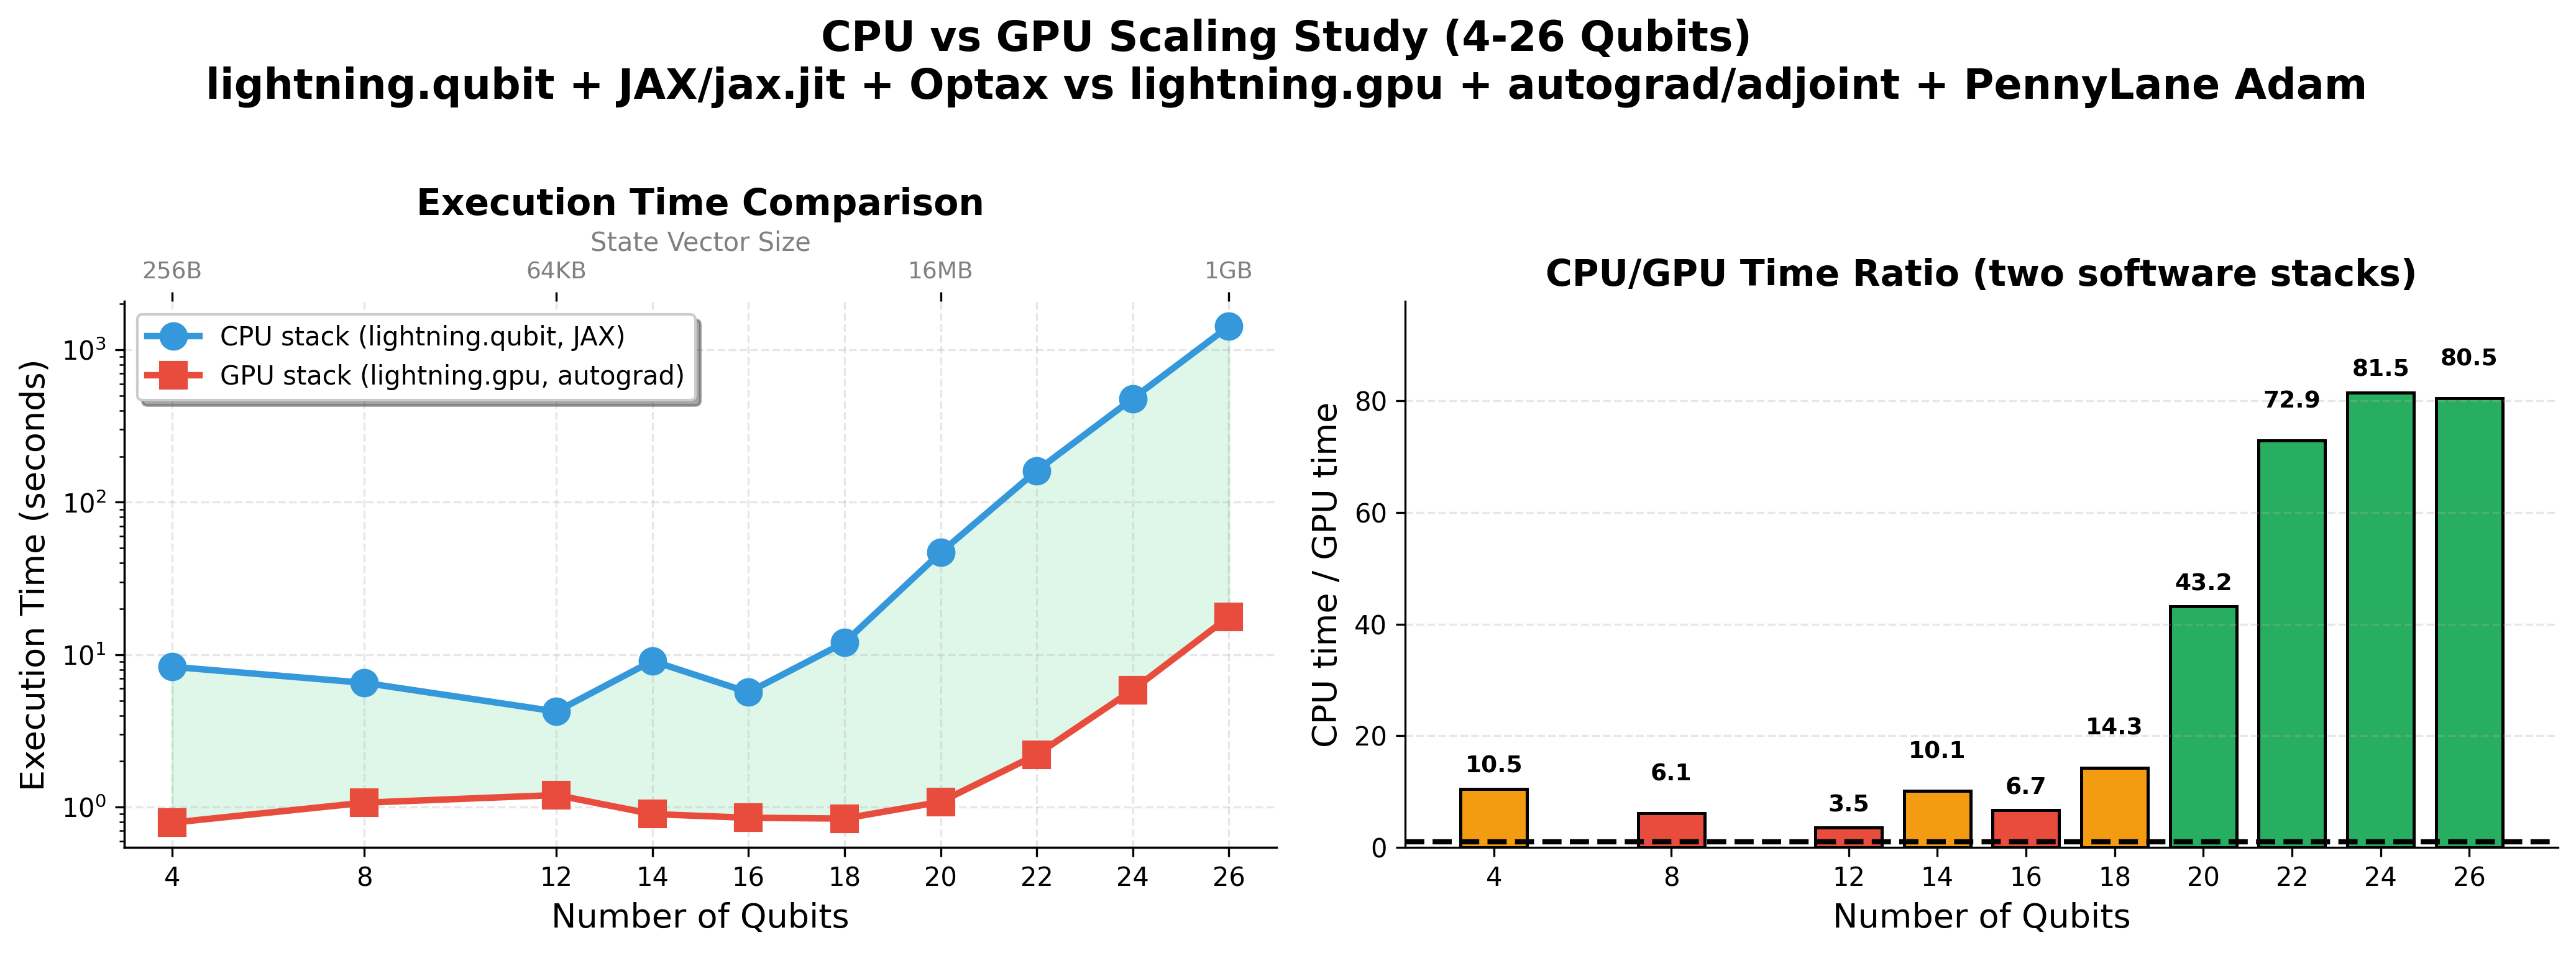
\includegraphics[width=\textwidth]{../results/scaling_study/scaling_comparison.png}
    \caption{CPU and GPU stacks in the scaling study from 4 to 26 qubits. Left: runtime (log scale). Right: CPU/GPU time ratio.}
    \label{fig:scaling_study}
\end{figure}

\subsubsection{Implementation 5: MPI Parallelization}

The MPI implementation (\texttt{vqe\_mpi.py}) splits the 100 bond lengths into contiguous blocks, one per rank, and each rank runs the Optax and Catalyst JIT runner of Implementation~2 on its block. Table~\ref{tab:mpi_results} lists the measured runtimes.

\begin{table}[h]
    \centering
    \begin{tabular}{rr}
        \toprule
        \textbf{Ranks} & \textbf{Runtime (s)} \\
        \midrule
        2  & 8.45 \\
        4  & 6.07 \\
        8  & 5.48 \\
        16 & 5.06 \\
        32 & 5.04 \\
        \bottomrule
    \end{tabular}
    \caption{MPI runtimes for the 100-bond-length scan. Each value is the elapsed time on rank 0, measured before the final gather.}
    \label{tab:mpi_results}
\end{table}

We do not report a parallel speedup for these runs. The serial Optax and JIT job requested one core (\texttt{ppn=1}), and the MPI jobs ran under separate allocations. The per-bond times of the serial run assign 73.5~s of work to rank 0 and 70.3~s to rank 1 at 2 ranks, while the measured 2-rank runtime is 8.45~s. A balanced split of the same work cannot explain this factor of 8.7, so the serial and MPI jobs had different resources available, for example the number of cores each process could use. The timer also covers rank 0 only. We cannot rerun both jobs under one allocation, so the ratio of their runtimes mixes the effect of the rank count with the effect of the allocation. Among the MPI runs, the runtime falls from 8.45~s at 2 ranks to 5.04~s at 32 ranks.

\subsubsection{Implementation 6: Multi-GPU Runs}

The multi-GPU benchmark uses a separate test problem: a sum of Pauli-$Z$ operators on $n$ qubits, a layer of $R_Y$ rotations (with an additional $R_Z$ layer in the maximum-size test) followed by a CNOT chain, \texttt{lightning.gpu} with adjoint differentiation, and gradient descent with step size 0.1. One MPI rank drives each GPU.

\textbf{Maximum size.} On one H100, 5 iterations at 26, 28, and 29 qubits take 0.62~s, 2.46~s, and 5.07~s per iteration. The 30-qubit run fails with an out-of-memory error. Figure~\ref{fig:multi_gpu} shows these times together with an estimate of the GPU memory, which we compute as four times the $2^n \times 16$-byte state vector. The estimate gives 64~GB at 30 qubits, below the 80~GB of the H100, so it undercounts the memory that \texttt{lightning.gpu} allocates.

\textbf{Independent problems.} In the scaling test, each of the 4 GPUs solves 2 independent 22-qubit problems with 15 iterations each. The longest per-GPU time is 8.04~s, and the sum of the four per-GPU times is 31.99~s. Their ratio, 3.98, shows that the four GPUs carried equal load. It is not a measured speedup, because we did not run the 8 problems on a single GPU. In the throughput test, each GPU solves 3 independent 20-qubit problems, and the longest per-GPU time is 12.27~s.

\begin{figure}[h]
    \centering
    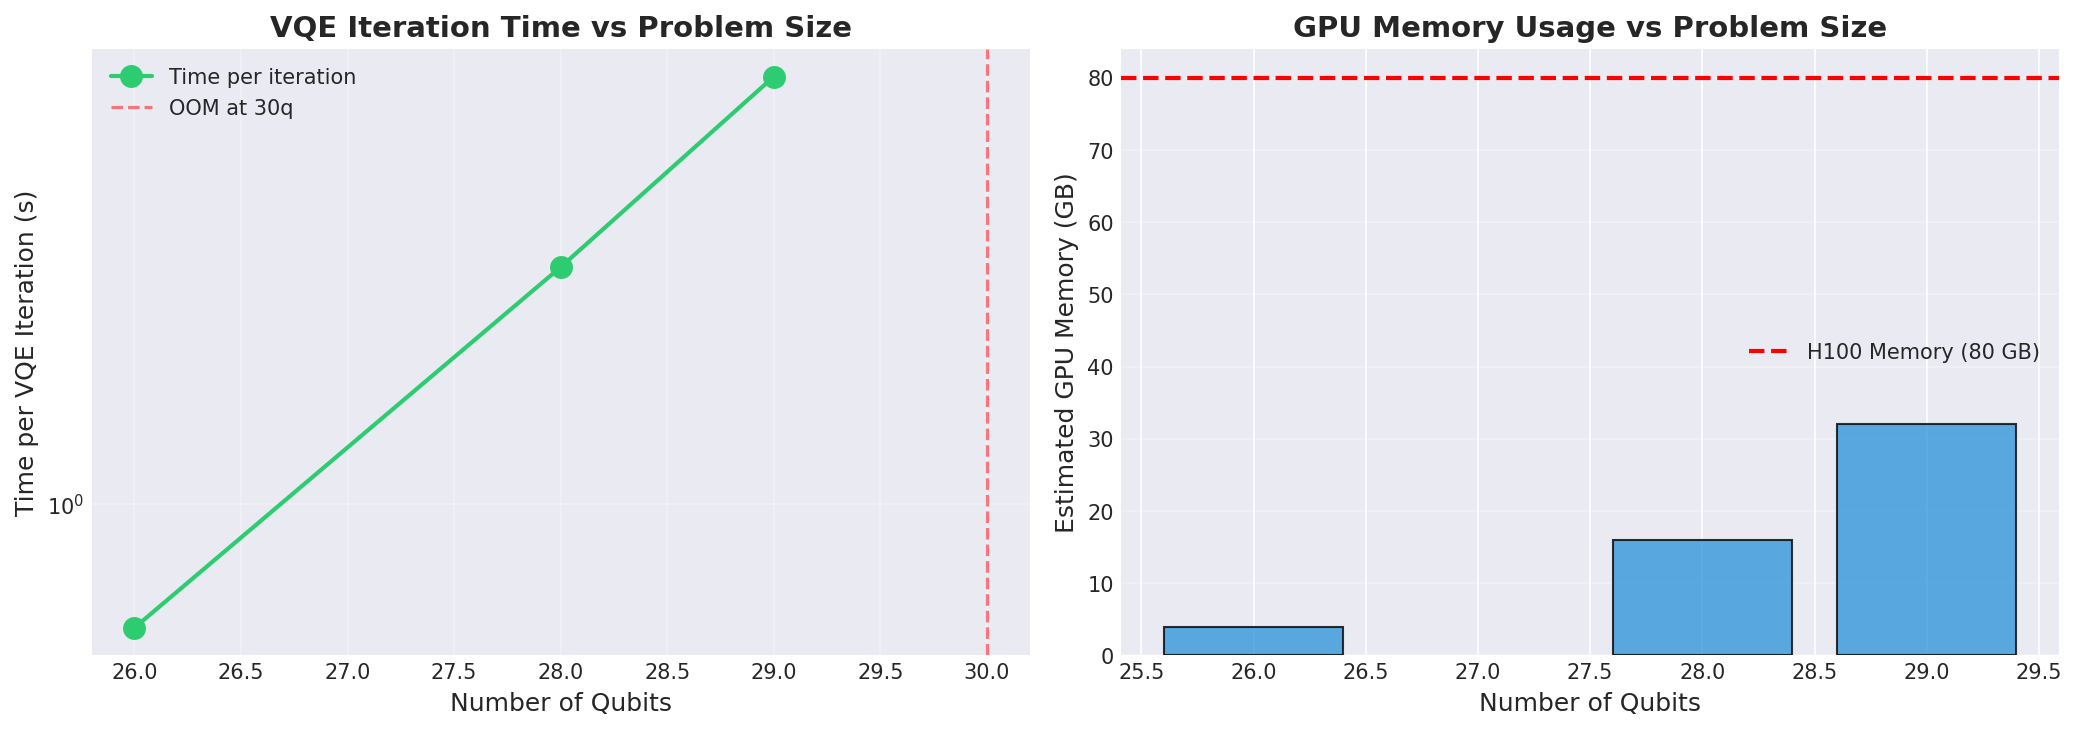
\includegraphics[width=\textwidth]{../results/multi_gpu/max_qubit_scaling.png}
    \caption{Maximum problem size on one NVIDIA H100. Left: measured time per iteration at 26, 28, and 29 qubits. Right: estimated GPU memory, four times the complex128 state vector. The 30-qubit run failed with an out-of-memory error.}
    \label{fig:multi_gpu}
\end{figure}

\section{Discussion}

\subsection{Physical Interpretation of Results}

The computed potential energy surface has the expected features of H$_2$. The grid values below come from the Implementation~2 run.

\textbf{Equilibrium Geometry:} The lowest energy on the grid lies at 0.725~\AA, and the next grid point is 0.752~\AA\ (grid spacing 0.027~\AA). The experimental bond length of 0.741~\AA\ lies between them.

\textbf{Equilibrium Energy:} The lowest VQE energy on the grid is $-1.137217$~Ha at 0.725~\AA. Exact diagonalization of the same STO-3G qubit Hamiltonian in the two-electron sector gives $-1.137221$~Ha, a difference of $4\times10^{-6}$~Ha.

\textbf{Dissociation Behavior:} Beyond 2.5~\AA, the energy approaches the separated-atom limit.

\textbf{Ansatz:} In the STO-3G basis, the ground state of H$_2$ lies in the span of the Hartree-Fock state $|1100\rangle$ and its double excitation $|0011\rangle$, because single excitations change the spatial symmetry. The single-parameter double excitation ansatz can therefore represent the exact STO-3G ground state at every bond length. Exact diagonalization at 0.35, 0.725, 1.5, and 3.0~\AA\ confirms that the ground state has unit weight in this two-dimensional span.

\textbf{HPC Focus:} These results check the VQE implementation. The rest of the paper treats the scan as an HPC workload.

\subsection{Computational Performance Analysis}

\textbf{Serial Baseline:} The preliminary serial run (Table~\ref{tab:serial_performance}) achieves 157.98 circuit evaluations per second. On the cluster, the baseline takes 593.95 seconds for 100 bond lengths with 300 iterations each.

\textbf{Bottleneck Identification:} We profiled a serial run with 10 bond lengths and 50 iterations with Python's \texttt{cProfile}. QNode calls (\texttt{qnode.\_\_call\_\_}), which include the gradient computation (\texttt{\_grad\_with\_forward}), take 28.2~s of the 32.7~s runtime (86\%). The Amdahl estimate in Section~\ref{sec:prediction} assumes a parallel fraction of 0.95, higher than this measured 0.86.

\textbf{Iteration Count:} On one core, the largest runtime reduction comes from fewer iterations. Early stopping, a larger learning rate, and warm starts cut the iteration count by a factor of 4.3 and the runtime by a factor of 4.13 (Implementation~2).

\textbf{GPU:} At 4 qubits, \texttt{lightning.gpu} has the lowest time per iteration (0.0145~s), but it runs 11,345 iterations from cold starts and finishes after the JIT run. In the scaling study, the GPU stack is faster at every size from 4 to 26 qubits, with a CPU/GPU time ratio between 3.5 and 81.5, for two stacks that differ in interface, differentiation method, and optimizer.

\textbf{MPI:} Runs with 2 to 32 ranks take between 8.45~s and 5.04~s. We do not compare them with the serial runs, for the reasons in Implementation~5.

\textbf{Multi-GPU:} One H100 runs up to 29 qubits. Independent problems spread evenly across 4 GPUs (sum of per-GPU times 31.99~s, longest per-GPU time 8.04~s). A single-GPU run of the same problems is needed to measure a speedup.

\subsection{Relevance to Original Questions}

\textbf{Question 1: VQE Accuracy}

VQE with a single-parameter double excitation ansatz computes the H$_2$ potential energy surface in the STO-3G basis, with an energy of about $-1.137$~Ha at the equilibrium bond length (Figure~\ref{fig:serial_pes}).

\textbf{Question 2: HPC Parallelization}

The H$_2$ scan parallelizes across bond lengths with no communication between ranks, and the MPI runs complete the scan in 5.04~s to 8.45~s. Our measurements do not isolate the parallel speedup, because the serial and MPI jobs ran under different allocations (Implementation~5). On one core, the stopping rule, learning rate, and starting point change the runtime by a factor of 4.13 while the time per iteration stays between 0.0198~s and 0.0204~s. For 20 to 26 qubits, the GPU stack in the scaling study runs 43.2 to 81.5 times faster than the CPU stack.

\section{Conclusions}

We implemented VQE for the hydrogen molecule potential energy surface and measured four implementations on the ERAU Vega cluster with 4 NVIDIA H100 GPUs:

\begin{enumerate}
    \item \textbf{Algorithm Validation:} The single-parameter double excitation ansatz reproduces the H$_2$ potential energy surface, with $\sim$-1.137~Ha at 0.74~\AA.

    \item \textbf{Iteration Count:} Early stopping, a larger learning rate, and warm starts reduce the iterations from 30,000 to 7,033 and the runtime from 593.95~s to 143.80~s. The time per iteration stays between 0.0198~s and 0.0204~s, so the reduction tracks the iteration count.

    \item \textbf{GPU:} At 4 qubits, \texttt{lightning.gpu} lowers the time per iteration to 0.0145~s. In the 4 to 26 qubit study, the CPU/GPU time ratio ranges from 3.5 to 81.5, for two software stacks that differ in interface, differentiation method, and optimizer.

    \item \textbf{MPI:} 2 to 32 ranks complete the scan in 8.45~s to 5.04~s. The serial and MPI jobs ran under different resource allocations, so we report no MPI speedup.

    \item \textbf{Multi-GPU:} One H100 runs up to 29 qubits, and 30 qubits fails with an out-of-memory error. Eight independent 22-qubit problems on 4 GPUs take at most 8.04~s per GPU, against a sum of 31.99~s over the four GPUs. We did not run them on one GPU.

    \item \textbf{Practices:} Report the optimizer, stopping rule, and starting point with each runtime, because these settings changed the runtime by a factor of 4.13 in our runs. Run the serial baseline and the parallel runs under one resource allocation, and time the slowest rank. Measure a single-device run before reporting multi-device efficiency.
\end{enumerate}

\subsection{Broader Impact}

The bond-length scan is a parameter sweep in which each point is an independent optimization. The same distribution across ranks or GPUs applies to other sweeps of this form, for example scans over several geometric parameters.

\section{Changes in Version 2}

Version~1 of this preprint attributed a 4.13$\times$ runtime reduction to JIT compilation, reported an MPI speedup of 28.5$\times$ and a combined speedup of 117$\times$, and reported 99.4\% multi-GPU parallel efficiency. Version~2 corrects these statements. The 4.13$\times$ reduction tracks a 4.3$\times$ reduction in iteration count from early stopping, a larger learning rate, and warm starts. The MPI speedups compared jobs with different resource allocations, and version~2 withdraws them; the measured MPI runtimes remain. The 99.4\% figure divided the sum of per-GPU times by four times the longest per-GPU time, so it measured load balance, not speedup. Version~2 also corrects the description of the scaling-study Hamiltonian (transverse-field Ising, not a sum of Pauli-$Z$ operators), states the software differences between the CPU and GPU paths, and removes the figure built on the withdrawn speedups. It also corrects three entries of the Amdahl prediction table, the bond-length range (0.35 to 3.0~\AA, not 0.1 to 3.0~\AA), and the baseline iteration count (300, not 200).

\section{Acknowledgements}

We thank Dr. Khanal for guidance on parallelization strategies and HPC methodologies. This work was conducted on the ERAU Vega HPC cluster featuring AMD EPYC 9654 processors and NVIDIA GPU accelerators. The quantum simulations used the PennyLane quantum computing framework with Lightning backend, JAX for automatic differentiation, and Catalyst for JIT compilation.

Large language model tools were used to assist with manuscript preparation and editing. The authors take full responsibility for all scientific content, methodology, and results.

\section{Codebase}

All source code can be accessed at https://github.com/rylanmalarchick/QuantumVQE

\begin{thebibliography}{99}

    \bibitem{peruzzo2014}
    A. Peruzzo, et al.,
    \textit{A variational eigenvalue solver on a photonic quantum processor},
    Nature Communications \textbf{5}, 4213 (2014).

    \bibitem{romero2018}
    J. Romero, R. Babbush, J. R. McClean, C. Hempel, P. J. Love, and A. Aspuru-Guzik,
    \textit{Strategies for quantum computing molecular energies using the unitary coupled cluster ansatz},
    Quantum Science and Technology \textbf{4}, 014008 (2018).

    \bibitem{kandala2017}
    A. Kandala, et al.,
    \textit{Hardware-efficient variational quantum eigensolver for small molecules and quantum magnets},
    Nature \textbf{549}, 242--246 (2017).

    \bibitem{bergholm2018}
    V. Bergholm, et al.,
    \textit{PennyLane: Automatic differentiation of hybrid quantum-classical computations},
    arXiv:1811.04968 (2018).

    \bibitem{pennylane_lightning}
    Xanadu,
    \textit{PennyLane-Lightning: Fast state-vector simulator},
    \url{https://github.com/PennyLaneAI/pennylane-lightning} (2024).

    \bibitem{cuquantum2023}
    NVIDIA Corporation,
    \textit{cuQuantum SDK: High-performance libraries for quantum computing simulation},
    \url{https://developer.nvidia.com/cuquantum-sdk} (2023).

    \bibitem{jax2018}
    J. Bradbury, et al.,
    \textit{JAX: Composable transformations of Python+NumPy programs},
    \url{https://github.com/google/jax} (2018).

    \bibitem{valiev2010}
    M. Valiev, et al.,
    \textit{NWChem: A comprehensive and scalable open-source solution for large scale molecular simulations},
    Computer Physics Communications \textbf{181}, 1477--1489 (2010).

    \bibitem{pennylane}
    V. Bergholm, et al.,
    \textit{PennyLane: Automatic differentiation of hybrid quantum-classical computations},
    arXiv:1811.04968 (2018).

    \bibitem{mcardle2020}
    S. McArdle, S. Endo, A. Aspuru-Guzik, S. C. Benjamin, and X. Yuan,
    \textit{Quantum computational chemistry},
    Reviews of Modern Physics \textbf{92}, 015003 (2020).

    \bibitem{cerezo2021}
    M. Cerezo, et al.,
    \textit{Variational quantum algorithms},
    Nature Reviews Physics \textbf{3}, 625--644 (2021).

    \bibitem{szabo1996}
    A. Szabo and N. S. Ostlund,
    \textit{Modern Quantum Chemistry: Introduction to Advanced Electronic Structure Theory},
    Dover Publications (1996).

    \bibitem{amdahl1967}
    G. M. Amdahl,
    \textit{Validity of the single processor approach to achieving large scale computing capabilities},
    AFIPS Conference Proceedings \textbf{30}, 483--485 (1967).

\end{thebibliography}

\end{document}
